\section{Analysis}

We begin our analysis with some information about the data
we are analyzing.
Our reduced statistics file includes over 25 million revision
records.
Figures~\ref{fig-revs-quality} and~\ref{fig-revs-contrib} were
created by drawing a random sample of 5 million records,
due to memory limitations of the software package.
%% CUT: Luca & Bo discussed this, and decided that it
%% would be distracting to the audience.  Since we're
%% already sampling 20%, most people won't take issue.
% ; three different samples of 5 million
% records produced nearly identical results.

In Figure~\ref{fig-revs-quality}, we show the frequency distribution
of the two quality measures
\quality{tdecay}{10}{} and \quality{elong}{10}{} over the revisions we sampled.
We see both measures are heavily biased towards $+1$, indicating that
most revisions to the Wikipedia are generally considered useful
by succeeding authors.
This confirms the intuition that more ``good people'' than
``bad people'' must contribute, otherwise the Wikipedia would
have a difficult time maintaining the community which
continues to extend the online encyclopedia in a useful way.
%
\begin{figure}[tbhp]
    \begin{center}
    \fbox{
    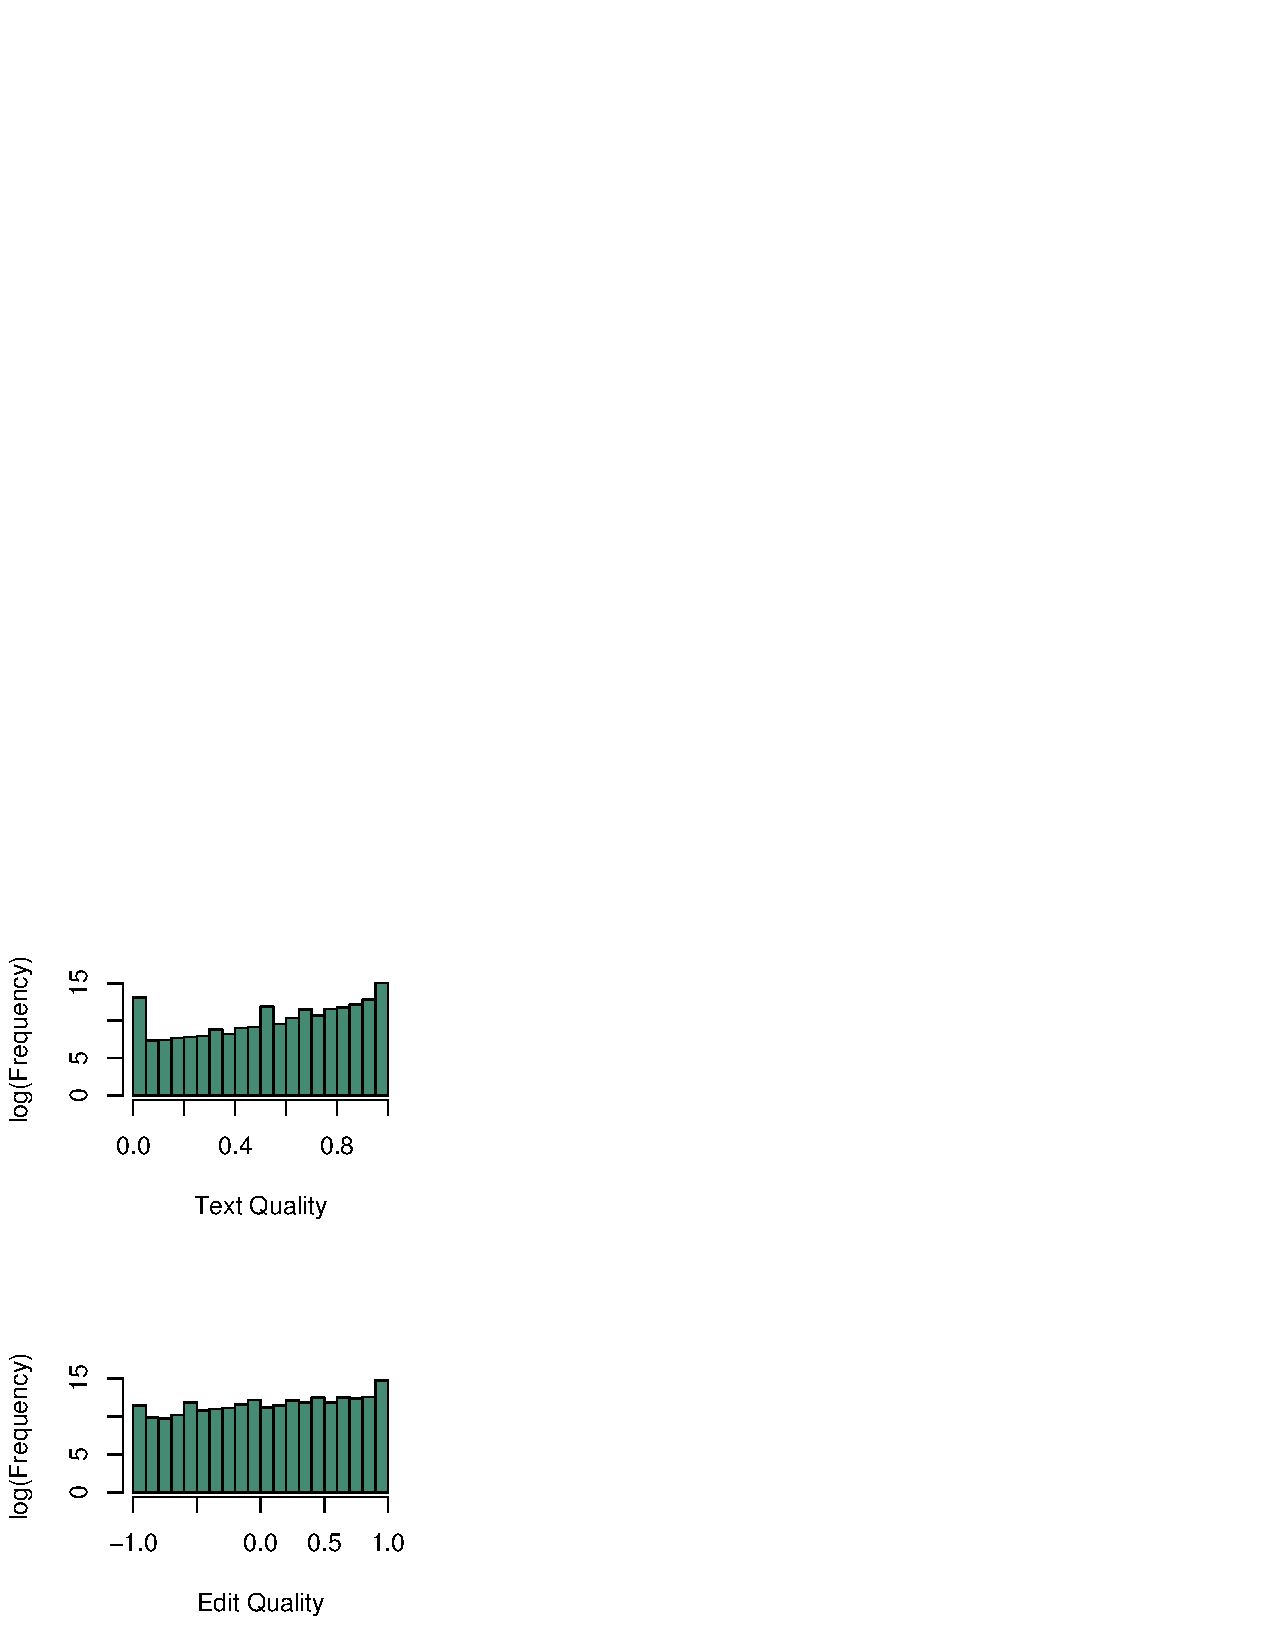
\includegraphics[width=0.70\textwidth]{part-I10-contrib/graphs/all_quality}
    }
    \end{center}
    \caption[Measuring edit and text quality over revisions]{
    	This graph shows the text quality $\quality{tdecay}{10}{}$
        and edit quality measure $\quality{elong}{10}{}$
	for 5~million randomly selected records of each type.
    }
    \label{fig-revs-quality}
\end{figure}

Delving directly into the data for text quality, we observe
that $10\%$ of the revisions made had
$\quality{tdecay}{10}{} \le 0.05$ while $66.67\%$ of the revisions had
$\quality{tdecay}{10}{} > 0.95$.
When $\quality{tdecay}{10}{} = 0$, the text is immediately deleted
in the next revision, so we can infer that these revisions
are the work of vandals.
When we look at the size of contributions made, we noticed that
$6\%$ of the amount of new text added had $\quality{tdecay}{10}{} = 0$,
whereas $76.21\%$ of the new text added had $\quality{tdecay}{10}{} > 0.95$.
From this we conclude that authors mostly add good new text.

The data is less stark for edit quality.
When we looked at revisions, we saw that $1.9\%$ of the revisions
had $\quality{elong}{10}{} \le -0.9$, whereas $51.12\%$ had
$\quality{elong}{10}{} > 0.9$.
In fact, $84.71\%$ had positive edit quality.
In terms of edit contributions, we noticed that $7.5\%$ of the
edit contributions had $\quality{elong}{10}{} \le -0.9$, whereas
$61.39\%$ had $\quality{elong}{10}{} > 0.9$.
Moreover, $1.6\%$ of the edit contributions were immediately
reverted.
From these statistics, we conclude that authors mostly do good
edits, but that contributions are massaged a bit by later editors.

Figure~\ref{fig-revs-contrib} shows the absolute text and edit
contributions, \txt{}{\version{i}} and \dist{}{\version{i}}, for the sets of sampled revisions.
It is important to note that these two graphs are using
the logarithm of the size of contribution, along the $x$-axis;
edit sizes can fall below $+1$, due to the way we compute
edit distance.
For moved words, they are included as a fraction of how much of
the document they move across;
if words are replaced with an equivalent number of words (as
can happen with synonyms replaced for clarity), the next contribution
to edit distance is zero.
Thus, the frequency count for edit sizes between $0$ and $1$
suggests that a good fraction of revisions involve rearranging
of text.
Beyond that, we can conclude that contributions, as measured
by text added or by edit distance, are predominantly under
100 words.
%
\begin{figure}[tbhp]
    \begin{center}
    \fbox{
    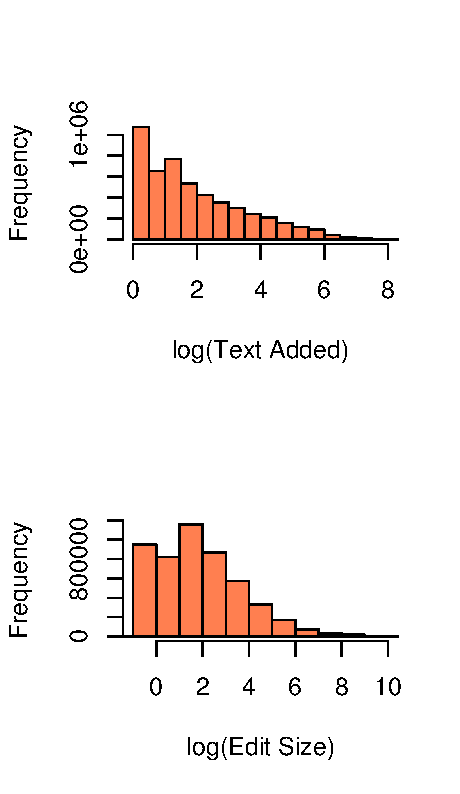
\includegraphics[width=0.70\textwidth]{part-I10-contrib/graphs/all_contrib}
    }
    \end{center}
    \caption[Measuring total edit and text contribution over revisions]{
        This graph shows the absolute text and edit contributions
        on a log scale, for 5 million randomly selected records
	of each type.
    }
    \label{fig-revs-contrib}
\end{figure}
%

In Figure~\ref{fig-user-quality} we show the average edit quality
and average text quality for all non-anonymous authors.
In order to compute this, we took all revisions created by each
author and took an average of the text and edit qualities of
those revisions.
We notice that $15.9\%$ of authors had $\quality{tdecay}{10}{} \le 0.05$
and $6.3\%$ of authors had $\quality{elong}{10}{} \le -0.9$.
These are shown by the bars on the left extreme of the
histograms in Figure~\ref{fig-user-quality}.
This sharp increase in the number of authors at the lowest end
of our quality measures, combined with our previous analysis
of revisions and contributions with respect to quality, gives
us some justification to define vandals as those
authors who have either $\quality{tdecay}{10}{} \le 0.05$ or
$\quality{elong}{10}{} \le -0.9$ on average.
We state that the identification of vandals can be made more
precise using more sophisticated analyses of our data, but we
don't deal with that in this paper.
%
\begin{figure}[tbhp]
    \begin{center}
    \fbox{
    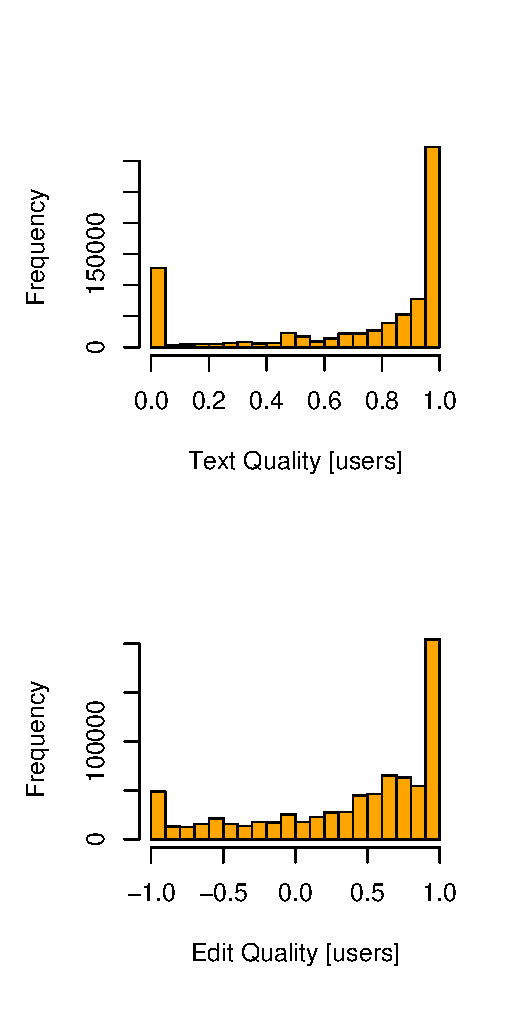
\includegraphics[width=0.60\textwidth]{part-I10-contrib/graphs/user_quality}
    }
    \end{center}
    \caption[Measuring edit and text quality for all authors]{
    	This graph shows the average text quality $\quality{tdecay}{10}{}$
	and the average edit quality measure $\quality{elong}{10}{}$
	over all non-anonymous authors.
    }
    \label{fig-user-quality}
\end{figure}
%

During our investigations comparing the proposed measures,
we found an unusually large fraction of non-anonymous authors
having scores relatively close to zero.
This suggested that many users had made a relatively
small number of revisions, and that the absolute
text and edit contributions of the revisions tended to
be small, or that the quality tended towards zero.
This is consistent with the power law distribution
for edits per author (Lotka's law) detected by~\cite{Voss2005};
we confirmed the distribution for our data (shown
in Figure~\ref{fig-hist-numedits}) and observed
that 362,461 authors made only one edit:
over 46\% of the total 777,223 authors we tracked.
In Figure~\ref{fig-singles-quality} we show the edit quality
measure for these authors.
In contrast to the edit quality distribution over
all authors from Figure~\ref{fig-revs-quality},
we notice that the edit quality for these authors
are almost evenly distributed across the
entire quality range (except for the two extreme values).
%
\begin{figure}[tbhp]
    \begin{center}
    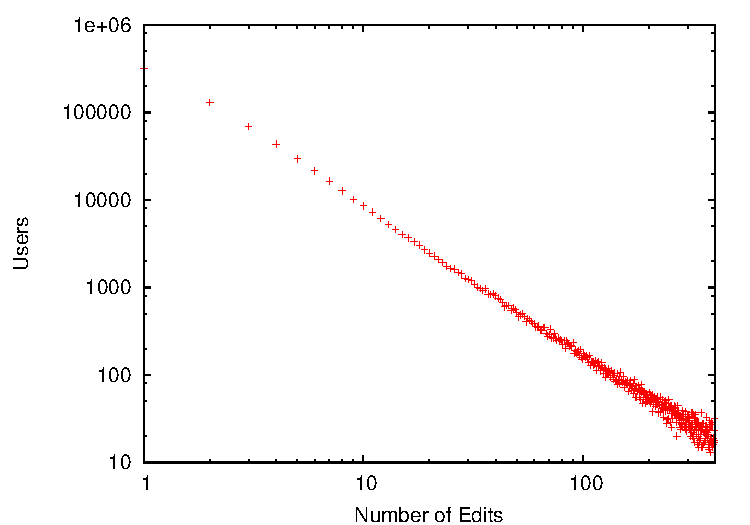
\includegraphics[width=0.75\textwidth]{part-I10-contrib/graphs/plot-hist-numedits}
    \end{center}
    \caption[Distribution of authors over number of edits]{
    	The distribution of the number of edits that each author made.
	Over 46\% of the non-anonymous authors
	make a single edit in the main English Wikipedia.
    }
    \label{fig-hist-numedits}
\end{figure}
%
\begin{figure}[tbph]
    \begin{center}
    \fbox {
    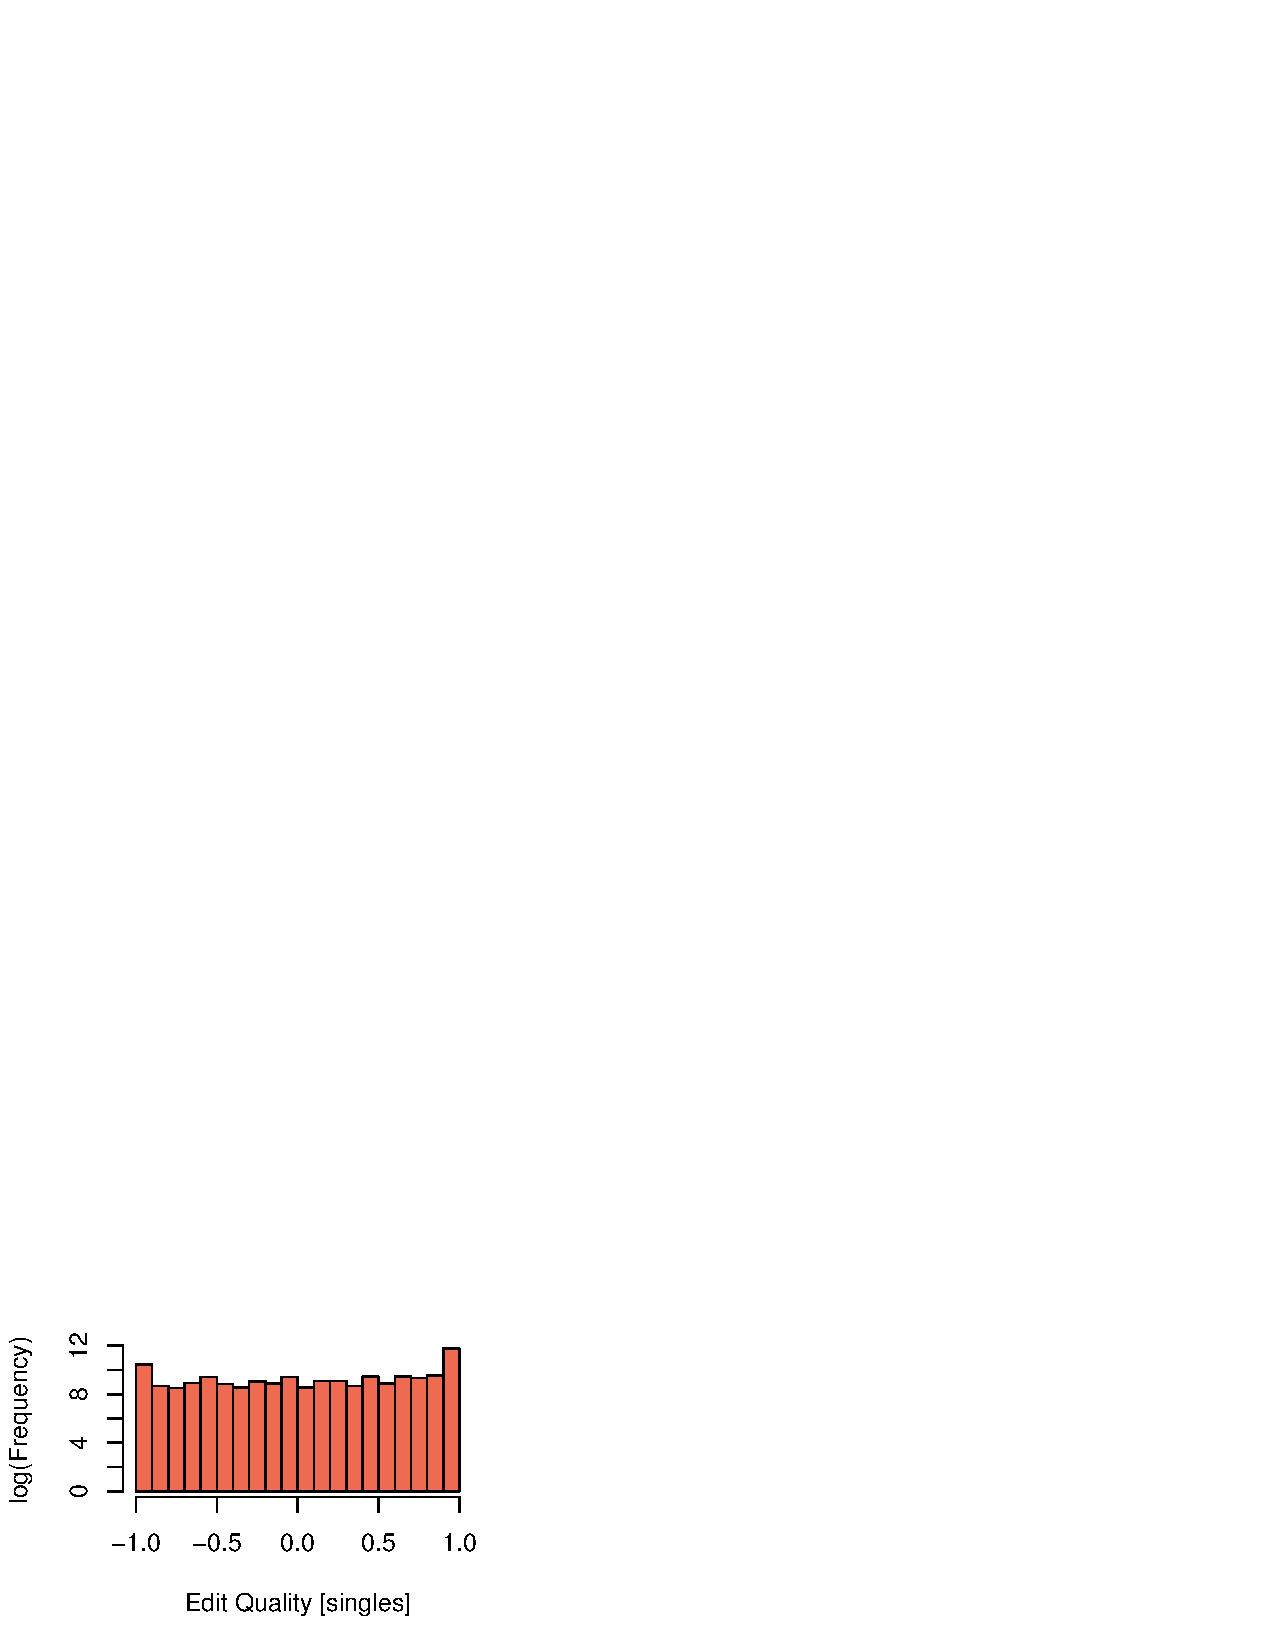
\includegraphics[width=0.70\textwidth]{part-I10-contrib/graphs/singles-quality}
    }
    \end{center}
    \caption[Edit quality of authors with one edit]{
        This plot shows the $\quality{elong}{10}{}$ of the
	non-anonymous authors who made a single edit contribution.
    }
    \label{fig-singles-quality}
\end{figure}

\pagebreak
\subsection{Comparing Measures}

We next present the correlations between the various measures
in Table~\ref{cor-tab}.
These are correlations with respect to the amount of contributions
made by all non-anonymous authors, excluding those we've classified
as vandals.  
% \mynote{Vishwa: why did we exclude vandals?  Maybe we
% should explain.  -Bo}
%
\begin{table*}[!tp]
\begin{center}
\begin{tabular}{|c||c|c|c|c|c|c|c|}
	\hline
$Measures$ &  $EditLong$ & $EditOnly$ & $NumEdits$ & $TenRevs$ & $TextLong$ & $TextOnly$ & $TextWPen$ \\
        \hline \hline
$EditLong$         &  1.000  & 0.999  &  0.28  &         0.070  & 0.075  &  0.16  & -0.32 \\
$EditOnly$         &  0.999  & 1.000  &  0.29  &         0.071  & 0.077  &  0.16  & -0.33 \\
$NumEdits$         &  0.283  & 0.286  &  1.00  &         0.361  & 0.417  &  0.45  &  0.27 \\
$TenRevs$          &  0.070  & 0.071  &  0.36  &         1.000  & 0.983  &  0.96  &  0.89 \\
$TextLong$         &  0.075  & 0.077  &  0.42  &         0.983  & 1.000  &  0.98  &  0.90 \\
$TextOnly$         &  0.158  & 0.164  &  0.45  &         0.963  & 0.983  &  1.00  &  0.82 \\
$TextWPen$         & -0.320  &-0.326  &  0.27  &         0.886  & 0.897  &  0.82  &  1.00 \\
        \hline
\end{tabular}
\end{center}
\caption[Correlations of our measures]{
This table gives the pairwise correlations of the different measures we 
have defined in this paper.
}\label{cor-tab}
\end{table*}
%
From the correlation table, we notice that text based measures are
better positively correlated with each other.
Similarly, the edit based measures are better positively correlated 
with each other as we expected.
The measures $\editlong$ and $\editonly$ are highly correlated as 
borne out by the fact that a large percentage of the edits are of
good quality.
We notice that the same is true for $\textlong$ and $\textonly$.
The correlation between $\punish$ and the absolute measure
$\editonly$ is low, demonstrating that $\punish$
penalizes authors for bad edits, gives no credit to good edits,
and accumulates the quality discounted text contribution measure 
$\textlong$.
Therefore, authors need to contribute high quality text, while
ensuring that they have no bad edits to get a high score on
$\punish$.
$\tenrevs$ being a text contribution measure, is highly correlated
with the other text contribution measures $\textonly$ and
$\textlong$.
$\numedits$ is positively correlated with all measures as we would
expect, since the majority of contributions are deemed good by
each of the quality measures.

While $\textonly$ and $\editonly$ appear to be reasonable measures 
of author contribution, we have found evidence that vandals
accrue large contributions against these measures.
For instance, we found that author $1065172$ is in the $99th$ 
percentile when measured using $\textonly$, but is nearly at the
bottom of the ranks, at $0.000001$ quantile when we look at his
$\punish$ measure.
We found five revisions in which this author added new text, but
four of those were immediately reverted.
The only revision that was kept around was a one word addition to a
page!
From the edits made by this author, we saw that he is a spammer.
On the other hand, using $\textlong$ instead of $\textonly$ we
noticed that the author was below the $25th$ percentile.
On the $\editlong$ measure, this author was below the 
$0.001$ quantile; among the lowest in rank.
Therefore, we argue that the measures that discount $\textonly$ and 
$\editonly$ by a text or edit quality measure are more indicative
of the ``useful'' work added to the Wikipedia.
We argue that $\numedits$ is not as good a measure, since 
vandals and bots can easily make large numbers of bad edits.

We present two figures, Figure~\ref{fig-zoom-editonly-editlong}
and Figure~\ref{fig-zoom-textonly-textlong},
which have been restricted to a region containing the
bulk of the data points.
In Figure~\ref{fig-zoom-editonly-editlong},
we see a vee shape, which separates the authors into
two groups: those that have positive edit quality and those
that have negative edit quality, as measured by $\avgeditquality$.
The worse the quality of edits made by authors the less they
accumulate of the $\editlong$ measure, whereas the $\editonly$
measure, being oblivious to edit quality, attributes the same
contribution to an author whose contributions persists as it 
does to an author whose contributions do not.
On the negative side of $\editlong$, there are points that represent
vandals, who edit large sections of existing pages, which are
then immediately reverted.
Clearly, $\editonly$ ranks some of these authors very highly,
whereas $\editlong$ is able to distinguish them and rank
them very low.

In Figure~\ref{fig-zoom-textonly-textlong},
we see a similar vee shape; in this case, $\textlong$
cannot go below zero as the text quality measure is always 
non-negative, so vandals, by our definition, receive no 
contribution.
As before, the measure that incorporates quality can 
distinguish vandals from non-vandals and attribute a contribution
measure to authors that is proportional to the merit of their
contribution.

Of the various measures we introduced, $\punish$ is perhaps the
one with the least tolerance, since by this measure, the only way
an author can accumulate contribution is by adding new
text that persists and by making edits that are judged to be
of good quality.
Further, this measure does not reward authors for good edits,
but penalizes them for bad edits.
In Figure~\ref{fig-zoom-textonly-textwithpunish}, we plot $\textonly$
against $\punish$.
We see the vee shape, with vandals falling on a noticeable line in
the fourth quadrant, that has no $\textonly$ contribution.
Since almost all new text added by vandals is immediate reverted,
and their edits always have low quality, we notice that they get
low negative $\punish$ contributions.
In fact, we noticed that the bottom ten authors by rank when
measured according to $\punish$ were all vandals with the exception
of $AntiVandalBot$.
We explain this in the subsection on bots.

\begin{figure}[t]
    \begin{center}
    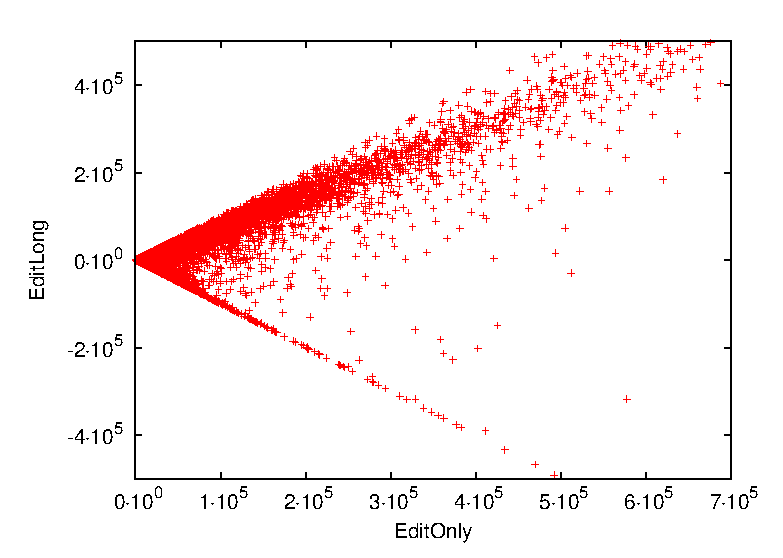
\includegraphics[width=0.45\textwidth]{part-I10-contrib/graphs/score-zoom-editonly-editlong}
    \end{center}
    \caption[EditOnly vs EditLong]{
    	Comparing the absolute edit contribution of a user
	with the edit longevity.
	Notice that authors who are ``all bad''
	are easily identifiable -- and sometimes quite prolific.
    }
    \label{fig-zoom-editonly-editlong}
\end{figure}
%
\begin{figure}[t]
    \begin{center}
    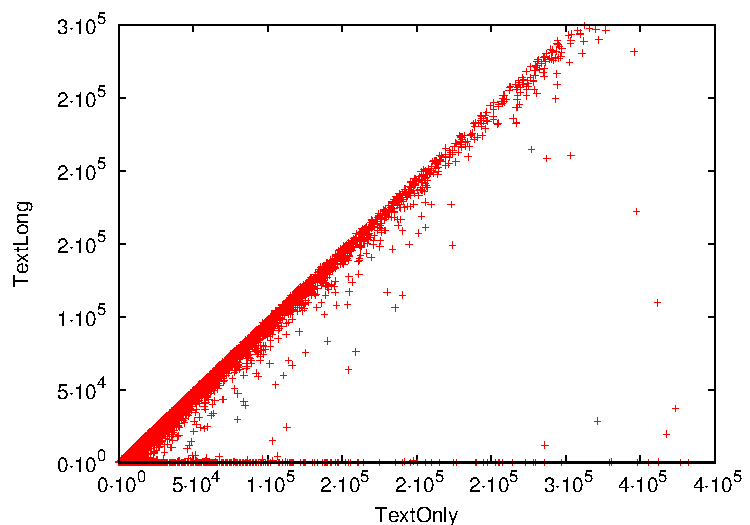
\includegraphics[width=0.45\textwidth]{part-I10-contrib/graphs/score-zoom-textonly-textlong}
    \end{center}
    \caption[TextOnly vs TextLong]{
    	Comparing the absolute text contribution with the contribution
	as measured by text longevity.
	We see that large contributors are either ``all bad''
	or nearly ``all good.''
    }
    \label{fig-zoom-textonly-textlong}
\end{figure}
%
\begin{figure}[t]
    \begin{center}
    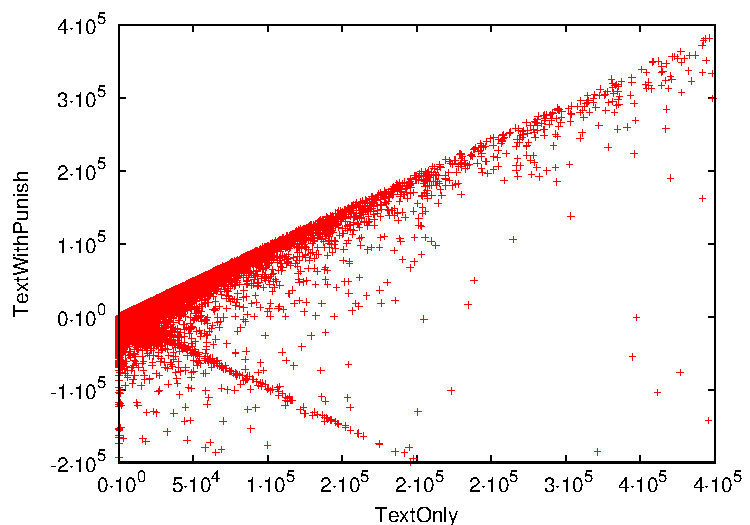
\includegraphics[width=0.45\textwidth]{part-I10-contrib/graphs/score-zoom-textonly-textwithpunish}
    \end{center}
    \caption[TextOnly vs TextWithPunish]{
    	Comparing the absolute text contribution of an author with
	their contribution as measured by \punish.
    }
    \label{fig-zoom-textonly-textwithpunish}
\end{figure}
%
\begin{figure}[t]
    \begin{center}
    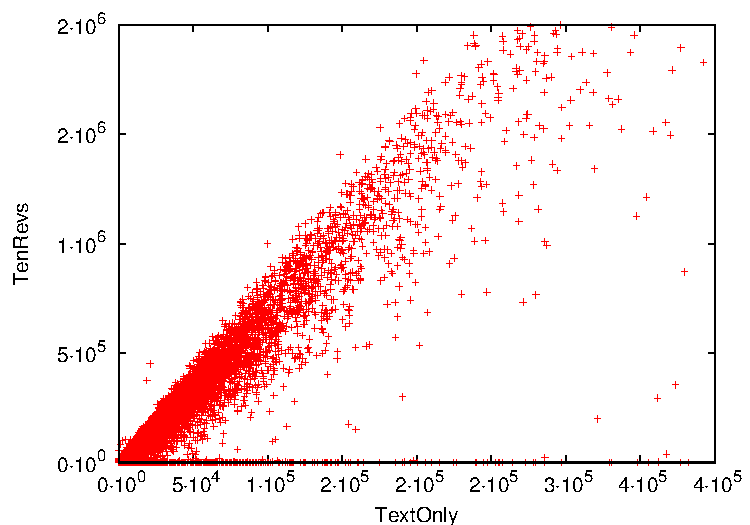
\includegraphics[width=0.45\textwidth]{part-I10-contrib/graphs/score-zoom-revisions-textonly}
    \end{center}
    \caption[Measuring short term text survival]{
    	This graph compares how much text is initially added
	by a user (along the $x$-axis), with how much
	of the text survives over the next ten filtered revisions
	(along the $y$-axis).
	The higher up the $y$-axis a point is, the more
	text that survived all ten revisions.
	Most authors add under 100,000 words,
	and about half of what they add survives.
    }
    \label{fig-zoom-revisions-textonly}
\end{figure}

\subsection{Ranking Authors}

A different direction we explored was how these different
measures end up ranking different authors.
Since the contribution measures varied over such a
wide range of values, with most people within
a smaller region around zero, we hoped that
ranking the authors would give us better insight into how
the measures differed.

To this end,  we computed the percentile rank
(rounded up to the next even value for clarity in the image)
of all non-anonymous authors, including those
that we had classified as vandals, and then plotted
them in 3-dimensional histograms; see
Figures~\ref{fig-prct-editlong-textlong}
and~\ref{fig-prct-editlong-textwithpunish}.
An important point to remember about
Figures~\ref{fig-prct-editlong-textlong}
and~\ref{fig-prct-editlong-textwithpunish}
is that the low-lying regions of the graph are
rarely zero --- there are roughly between one and ten
authors at each intersection, but this is so small compared
to the areas that correlate that we cannot see it on the graph.
Both figures show a high degree of correlation that wasn't evident
from the correlation scores in Table~\ref{tab:measure-correlations}.
Figure~\ref{fig-prct-editlong-textlong} shows that \textlong and
\editlong generally agree in the ranking of users, except for the lowest
scorers of \textlong.
The lowest scorers of \textlong all receive a score of zero, but the
``fence'' seen in the figure is an indication of the fact that there are
an enormous number of users which \textlong ranks equivalently but
\editlong is able to further distinguish between.
By contract, Figure~\ref{fig-prct-editlong-textwithpunish} shows that
\punish roughly agrees with \editlong for all users except for a thin
branch that score zero under \punish but get a positive score under
\editlong.
This thin branch represents the group of users which do not add text,
but instead only rearrange it or delete vandalism.
%
\begin{figure}[tbhp]
    \begin{center}
    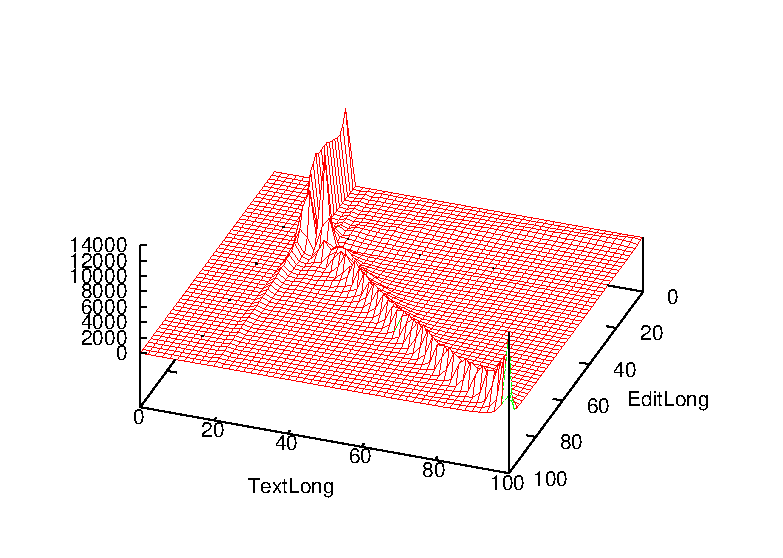
\includegraphics[width=0.85\textwidth]{part-I10-contrib/graphs/prct-editlong-textlong}
    \end{center}
    \caption[Comparing edit longevity with text longevity]{
    	$\editlong$ vs $\textlong$
    }
    \label{fig-prct-editlong-textlong}
\end{figure}
%
\begin{figure}[tbhp]
    \begin{center}
    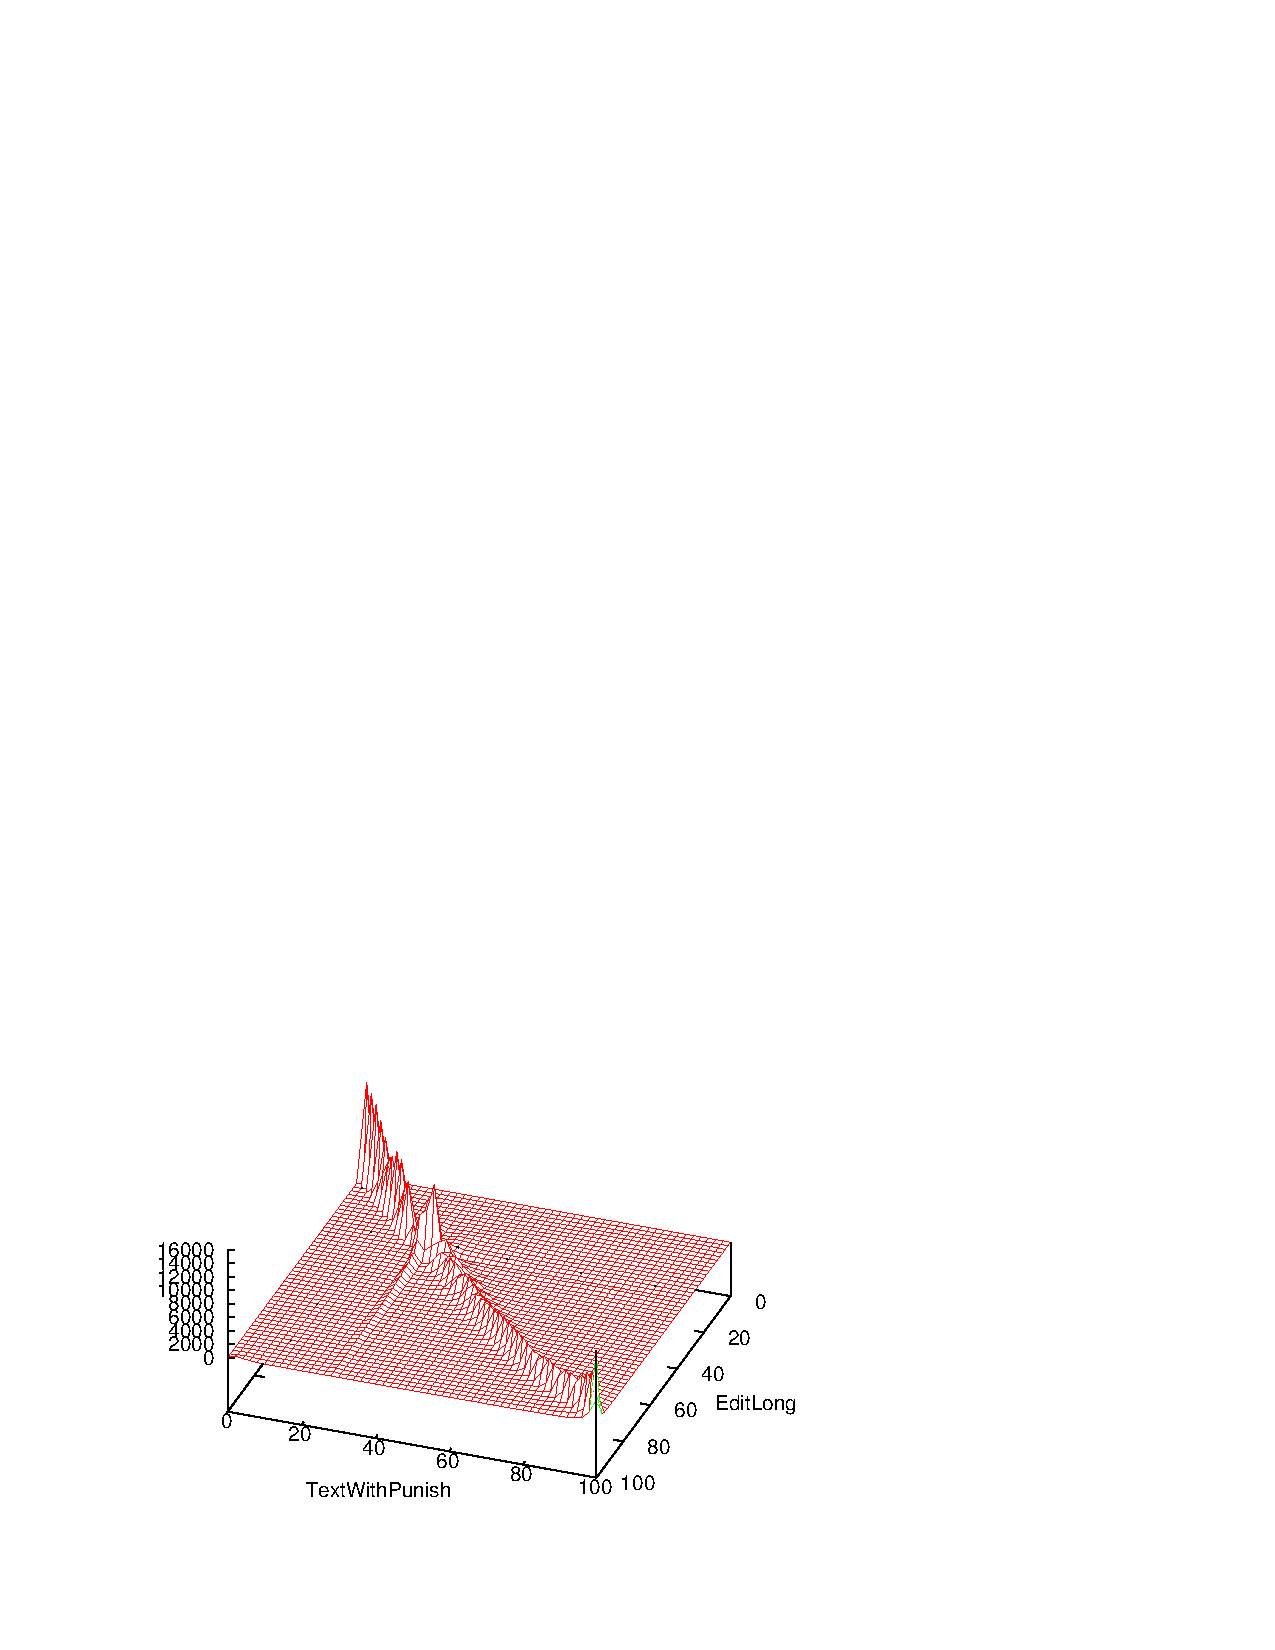
\includegraphics[width=0.85\textwidth]{part-I10-contrib/graphs/prct-editlong-textwithpunish}
    \end{center}
    \caption[Comparing edit longevity with the punishing function]{
    	$\editlong$ vs $\punish$
    }
    \label{fig-prct-editlong-textwithpunish}
\end{figure}
%

We also include a 3-dimensional histogram comparing the
percentile rankings as determined by \editlong and \numedits,
in Figure~\ref{fig-prct-editlong-numedits}.
The ``rows of fences'' we see
in Figure~\ref{fig-prct-editlong-numedits}
are due to the large number of authors who
make only a handful of edits; the \numedits measure
neither distinguishes them from each other,
nor is it capable of distinguishing good contributions from
bad contributions.
This last point is important, that even users in
the lowest percentile of \editlong can be rated
very highly by \numedits --- demonstrating
that it is much easier to game the \numedits
measure to achieve a high rank, while doing bad work.
%
\begin{comment}
%
\begin{figure}[tbhp]
    \begin{center}
    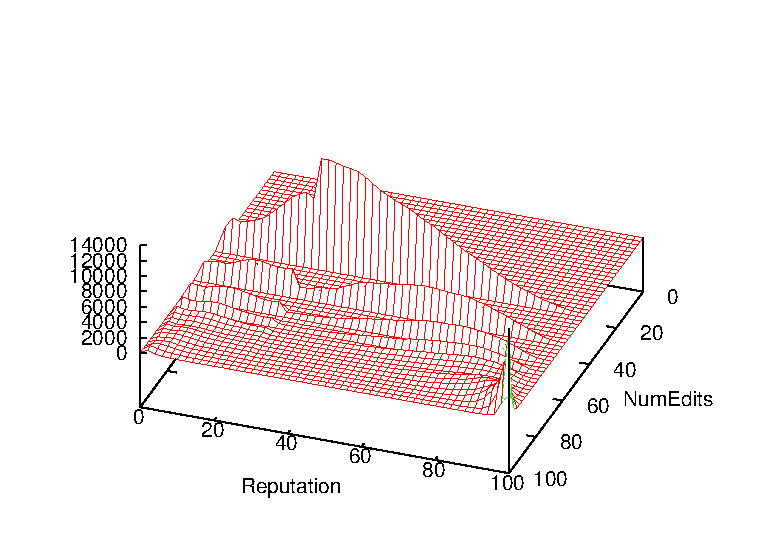
\includegraphics[width=0.85\textwidth]{part-I10-contrib/graphs/prct-numedits-reputation}
    \end{center}
    \caption[Comparing the number of edits made with the reputation function]{
    	The \contribrep measure had the highest correlation to \numedits,
	in Table~\ref{tab:measure-correlations}.
	Notice that \numedits does not distinguish well
	between users.
    }
    \label{fig-prct-numedits-reputation}
\end{figure}

\begin{figure}[tbph]
    \begin{center}
    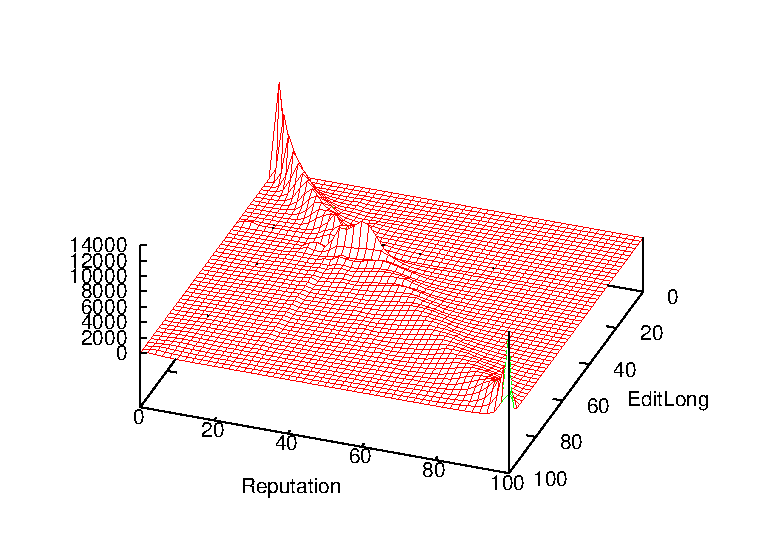
\includegraphics[width=0.85\textwidth]{part-I10-contrib/graphs/prct-editlong-reputation}
    \end{center}
    \caption[Comparing edit longevity with reputation]{
    	\editlong vs \contribrep
    }
    \label{fig-prct-editlong-reputation}
\end{figure}
%
\end{comment}

\begin{figure}[tbph]
    \begin{center}
    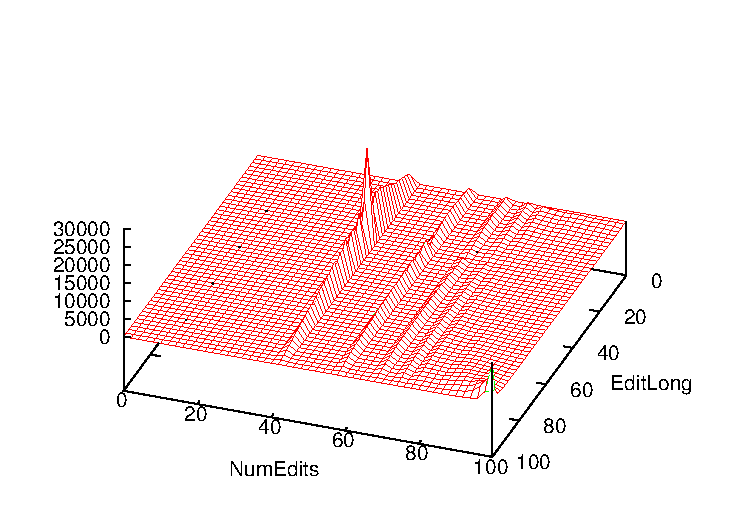
\includegraphics[width=0.85\textwidth]{part-I10-contrib/graphs/prct-editlong-numedits}
    \end{center}
    \caption[Comparing edit longevity with the number of edits made]{
    	$\editlong$ vs $\numedits$
    }
    \label{fig-prct-editlong-numedits}
\end{figure}


\subsection{Bot Behavior}

There are several bots operating on the contents of the Wikipedia.
Many bots are sanctioned by the community, and do useful
chores such as automatically removing text which is likely
to be vandalism, correcting spelling, and adding geographical data.
There are also bots which are created to vandalize pages,
and sometimes well-intentioned bots run amock and
accidentally vandalize pages as well.
During the course of comparing the various contribution
measures with each other, we found several bots (both
good and bad) which were obvious outliers in the data.
To analyze bots as a group, we selected all users
which included the ``Bot'' moniker in their username;
this self-identification does include some malicious bots,
but obviously favors selection of good bots.

The edit and text quality measures for all bots are similar to
that of all authors shown in Figure~\ref{fig-revs-quality}.
We noticed that bots create a large number of revisions with
high quality.
We found that $69.56\%$ of the revisions made by
bots have a text quality measure of $\textquality > 0.95$.
The percentage of revisions made by bots with 
$\textquality \le 0.05$ was $9.2\%$.
We found that $66.92\%$ of the new text added by bots were with
$\textquality > 0.95$ and $14.14\%$ of the new text added by
bots were with $\textquality = 0$, which means they were 
immediately reverted.
Similarly, on the edit contributions of bots we found that
$54.42\%$ of the revisions with edits made by bots were of
high edit quality, with $\avgeditquality > 0.9$.
The number of revisions having $\avgeditquality < -0.9$ being
negligible; $1\%$ from our analysis.
When we counted all edit revisions that had a negative edit
quality we saw that $12.73\%$ of the revisions were judged to 
be of poor quality with $\avgeditquality < 0$.
We found that $93.3\%$ of the edit contributions made by bots
had positive edit quality and the remaining $6.4\%$ had
negative edit quality.
More interestingly, $65.20\%$ of the edit contributions made
by bots had $\avgeditquality > 0.9$, which means they were
not edited out in subsequent revisions and represent the
sheer amount of work done by bots that is of very high quality.
The contributions with $\avgeditquality < -0.9$ are $1.8\%$.
This indicates that a large part of the text additions made by bots 
and a large part of the edit contributions made by bots survive
indefinitely.

Furthermore, our analysis indicates that bots make large amounts of
edit contributions compared to text contributions; the ratio
of the size of edits $\editonly$ to the size of new text $\textonly$
for all bots is $11.61$.
Since the penalizing measure $\punish$ does not credit authors for
good edits but reduces their $\textlong$ contributions, by the 
amount of their bad edits as measured by $\editlong$, we notice that 
edits judged as being of poor quality overwhelm the smaller text 
contributions of bots in general, and $AntiVandalBot$ in particular, 
resulting in a small overall contribution.
We also note here that $SmackBot$ did much better on this
measure.
$SmackBot$ contributes more text than $AntiVandalBot$.
Most of its edits are of smaller size than $AntiVandalBot$.
Since they have similar quality measures, $AntiVandalBot$ ends
up with a lower score on $\punish$ when compared to $SmackBot$.

\begin{comment}
%
\begin{figure*}
    \begin{center}
    \fbox{
    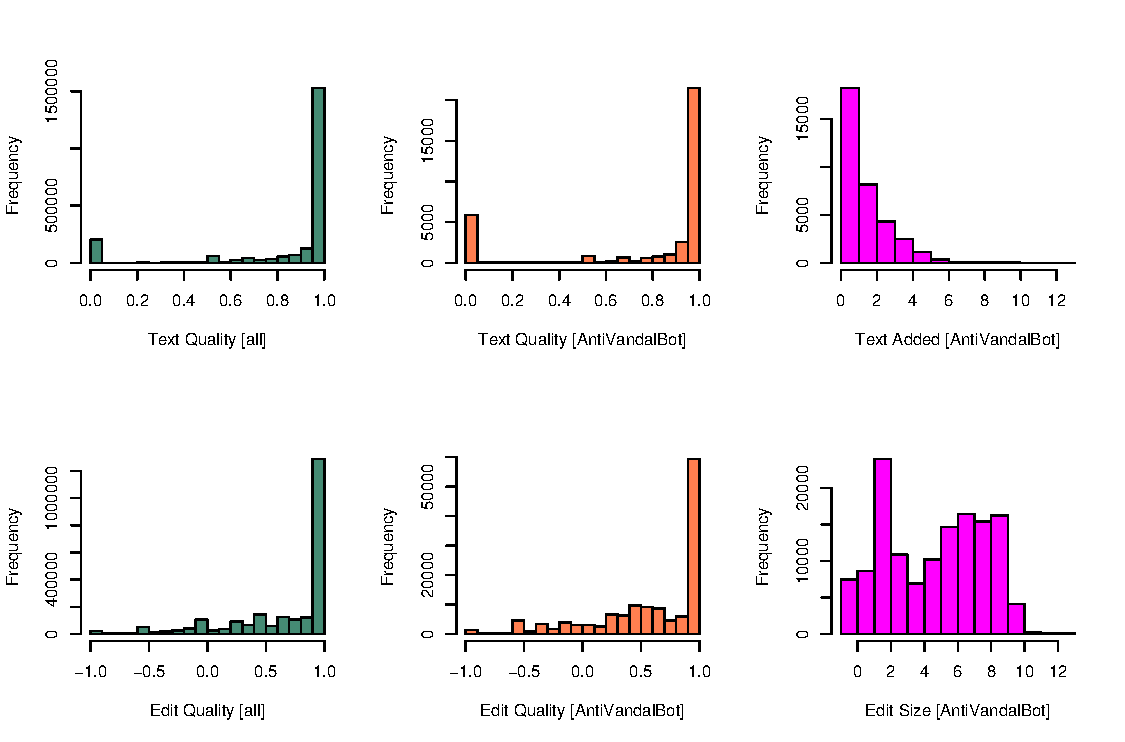
\includegraphics[scale=0.75]{part-I10-contrib/graphs/allbots_anti_hist}
    }
    \end{center}
    \caption[Measuring edit and text quality for all bots and $AntiVandalBot$]{
    	This graph shows the edit quality measure $\avgeditquality$
        and text quality $\textquality$ for all bots.
        A quality measure of $1$ indicates that all the changes
        were preserved.
        A quality measure of $0$ indicates that all the changes
        were reverted in the very next revision.
        The histograms on the left are for all bots.
        The ones on the right are the quality measures and the absolute amounts
        of text and edit contributions for $AntiVandalBot$.
    }
    \label{bot-contribs}
\end{figure*}
\end{comment}

\subsection{Sources of Error}

Since we use filtered revisions, namely we collapse all consecutive
revisions by the same author, and since we treat all anonymous authors
identically, consecutive edits made by anonymous authors cannot be
distinguished.
We therefore discard all anonymous authors from our analysis: in any
case, we are not measuring their contributions, as they cannot be
individually attributed. 
We have noticed that there are anonymous authors who do good work
on the Wikipedia, but at this point we have not implemented a
mechanism to attribute them a contribution measure.

We ignore the time difference between edits.
When pages receive many views with little editing, it suggests 
that the article is substantially correct;
perhaps later edits are due to changing facts, and not because 
of poor quality.
Articles which are the subject of current events are 
particularly likely to have their edit quality misjudged.
Relatedly, grouping revisions by author ignores the fact that 
edits separated by days or months are less related and have most 
likely been reviewed by others.




\subsection{Comparing Contributions}

Defining multiple contribution measures affords us
the opportunity to examine and quantify the
user behaviors over the large scale of edits performed.
We looked at the list of all blocked authors.~\footnote{Retrieved
on May 8, 2008, directly from the Wikipedia database.
It corresponds to the data available at
\url{http://en.wikipedia.org/wiki/Wikipedia:List_of_banned_users}.}
We separated them from the others with the objective of determining
how many of these authors met our definition of vandals.
We were surprised to note that over $51\%$ of authors had
$\quality{tdecay}{10}{} > 0.95$ and $39\%$ of authors had
$\quality{elong}{10}{} > 0.9$.
In fact, over $47\%$ of the blocked authors make text contributions
that have an average text quality over $0.95$.
Similarly, over $32\%$ of the these authors make edit contributions
that have an average edit quality over $0.9$.
We note that $11.2\%$ of these authors qualify as vandals by our measure,
based on their average edit quality and $24.9\%$ qualify as vandals
based on their average text quality.
But a large percentage of the authors in the blocked authors
list are not vandals, as determined by our definition.

A couple of cases in point are those of authors $3362$ and
$10784$.
They are both blocked, but are over the $99th$ percentile on
\editlong, \textlong and \punish.
One was blocked by Jimbo Wales and the other was blocked as he
was suspected of using multiple accounts.

We end this subsection, by mentioning the top rankers against all
measures.
The highest ranks across all contributions were secured by
authors $3903$ and \textit{AntiVandalBot}.
Author $3903$ had the top rank with respect to measures
\textonly, \textlong, \punish and \tenrevs.
\textit{AntiVandalBot} had the top rank with respect to the measures
\editlong and \editonly.
Interestingly, \textit{SmackBot} was the second highest scorer after
author $3903$ on measures \textlong and \punish.

